\chapter{Proposed solution}
\label{ch:proposed_solution}

In this section I will deliberate the proposed model background and its main dissemblance from general unet architecture.

Jointly the solution it was utilized 2 convolution networks with same architectures but sundry purposes and parameters. By scenario firstly it is issued detection model afterwards identification model. The detection model comes up with segmenting of vertebra from background. Whereas the identification model identifies what vertebrates belong which segmented pixels. To fine it down the identification model does not categorize each pixel in discrete manner, vice continuously produce value which subsequently is rounded correspondingly to a specific vertebra. It worth to mention inwardly full solution captures both short-range and long range information. Short-range information is retrieved utilizing detection model. The identification model is trained by feeding in large slices which capture long-range information which is essential for the task of identifying individual vertebrae. Acquisition of final results is done by multiplying detection and identification models results to elaborate labels on each pixel afterwards aggregating them to produce final centroid estimates for each vertebra.

The step by step representation in terms of visualisation is demonstrated on the figure \ref{fig:detection_identification_steps}.

\begin{figure}[h]
    \centering 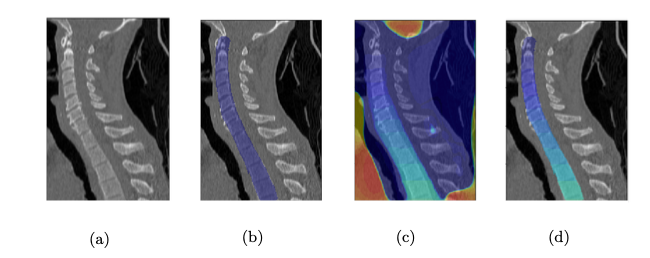
\includegraphics[width=12cm]{images/detection_identification_steps.png}
    \caption {(a) shows an original scan in grey-scale, (b) shows the output of the detection model applied to the scan, (c) shows the output of the identification model applied to the scan, (d) shows (b) and (c) multiplied together to produce a final prediction for each pixel.}
    \label{fig:detection_identification_steps}
\end{figure}

The chain of steps will not be capable if there would not be included background pixels in the identification stage therefore segmenting out the background in the detection step.


\section{Dataset}
The \href{https://biomedia.doc.ic.ac.uk/}{\color{blue}"BioMediaA"} database provide spine-focused CT scans of 125 patients with different types of pathologies. In total dataset consists of 242 scans. Each scan was manually annotated in terms of vertebrae centroids. 

Eventually data set was splitted into dedicated training (with ground-truth labels) and test sets each 242 and 60 scans accordingly. The scans were re-sample at $1mm \cdot 1mm \cdot 1mm$ resolution meaning each pixel in the generated samples from the scans provided a 3 dimensional $1mm$ section of the patient spine.

In the case of the detection model the dense labelling contains two values: 0 representing background and 1 representing vertebrae. The identification model’s dense labelling contains values from 0 to 26. Whilst 0 representing background, 1 representing C1 vertebrae up to 26 representing S2 vertebrae.

\begin{figure}[h]
    \centering 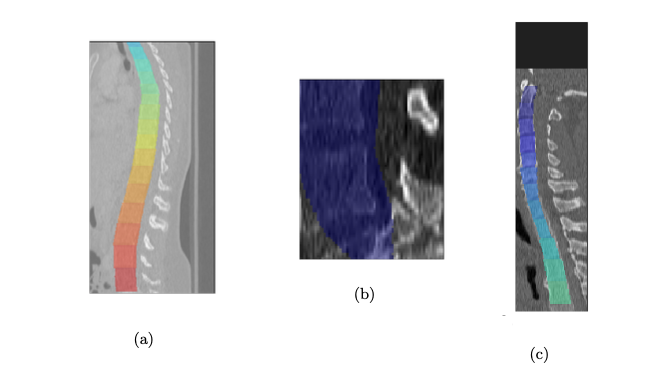
\includegraphics[width=10cm]{images/labeled_data.png}
    \caption {(a) shows a dense labelling, (b) shows an example of a sample used to train the detection model, (c) shows an example of a sample used to train the identification model. Note: The size of the sample is 8 x 80 x 320, if the original scan is not larger enough to fill those dimensions some padding is added, as can be seen at the top.}
    \label{fig:labeled_data}
\end{figure}

\newpage
\section{Metrics}
As for metrics I utilized Dice score, Id rate, mean localization distance and standard deviation (std) distance. Dice score measures goodness of predictions matched the training annotated ground truth segmentation, Id rate is the percentage of the centroid estimations predicted which are closest to the correct ground truth vertebra centroid (and are less than 20mm from that centroid). Mean and Std relate to the localization
error distance between the predicted centroid positions and the ground-truth centroid positions for the same vertebrae (if it occurs in the scan).

\subsection{Dice score}
Recall the \cite{Thada2013} Dice similarity coefficient (Dice score) was used to quantify how closely identification predictions matched the training annotated ground truth segmentation. 

Assume we annotated some ground truth region in particular image and then make an automated algorithm to do it so far. To validate the algorithm it is calculated Dice score, which is a measure of how similar the objects are. In other words it is the size of the overlap of the two segmentations divided by the total size of the two objects. As for mathematical representation it is formed as:
\begin{align*}
  \text{Dice score} = \frac{2\cdot|A\cap B|}{2\cdot|A\cap B| + |B\backslash A| + |A\backslash B|}
\end{align*}

\subsection{ID rate}
It was employed id rate measurement to validate correctness of closeness of predicted centroid estimations with ground truth vertebra centroid. The correctness measure actually is considered as a distance and was calculated for predicted and ground truth vertebrae centroids accordingly as:
\[ dist = ||A||_F = [\sum_{i,j} \abs(a_{i,j})^2]^{1/2} \]

Afterwards it was compared with predefined threshold as:
\begin{align*}
\begin{cases}
\lvert \text{dist} \rvert\ \mbox{if } \text{dist} \leq \text{min dist} \\ 
\text{skip}, \mbox{ otherwise} \end{cases}
\end{align*}

\subsection{Localization error}
As for localisation error if centroid occurs at the scan it was deliberated by mean and std of distance of localization error between predicted centroid position and ground-truth centroid position for particular vertebrae. Localization error notion is such as:
\[ \sum_{k=1}^K \frac{||\hat{\zeta_k} - \zeta_k || }{K} \]
where $K$ is the source number, $\hat{\zeta_k}$ and $\zeta_k$ are the estimated location and the real location of the $k$-th source, respectively.

\section{Loss function}
Shortly put, loss function is a function that maps an event or values of one or more variables onto a real number intuitively representing some "cost" associated with the event. 

Typically, with neural networks, we seek to minimize the error. As such, the objective function is often referred to as a cost function or a loss function and the value calculated by the loss function is referred to as simply loss.

\subsection{Weighted Categorical Cross Entropy}
Categorical Cross Entropy stands for quantifying multi-class classification tasks. As it all, it evaluates the difference between two probability distributions. Mathematically, categorical cross entropy has following notion: \[\text{Categorical Cross Entropy} = - \sum_{i-1}^{\text{output size}} y_i \cdot \log \hat{y_i} \]

Within the detection model it was used modified version of categorical cross entropy such as weighted categorical cross entropy. Mathematically loss function is defined as:

\begin{align*}
 L(P, Q) = P(0)\log Q(0) + P(1)\log Q(1)
\end{align*}
where $P$, $Q$ - particular distributions. 

By the reason the background label and vertebrae labels were issued with additional weights coefficients as $0.1$ and $0.9$ accordingly to reflect the proportion of background labels in the samples, the modified weighted categorical cross entropy was defined as:
\begin{align*}
 L(P, Q) = 0.1 \cdot P(0)\log Q(0) + 0.9 \cdot P(1)\log Q(1)
\end{align*}
where $P$, $Q$ - particular distributions.  

\subsection{L1}
L1 loss function stands for Least Absolute Deviations. It is used to minimize the error which is the sum of the all the absolute differences between the true value and the predicted value.

\[ \text{L1} = \sum_{i-1}^n |y_{true} - y_{predicted}|\]

The identification model does not classify each pixel discretely but instead produces a continuous value for each pixel. This value is then rounded to an integer which corresponds to a specific vertebra, for example $4 = C4$ vertebra. This means I may use an L1 loss function on each pixel and thus capture the ordering through this loss function. For that I have used the modified version of L1 loss function: 
\begin{align*}
 L1 = \begin{cases} \lvert y_i - x_i \rvert\ \mbox{if } x\mbox{$\neq 0$} \\ 0, \mbox{ otherwise} \end{cases}
\end{align*}
where $y_i$ - predicted value of pixel $i$ and $x_i$ - true value of pixel $i$.


\section{Detection Model}
As previously mentioned detection model showed on Figure \ref{fig:detection_model} comes up with segmenting of vertebra from background. Taking it closer into consideration the model classifies each dedicated pixel of scan whether it is background or vertebrae. Jointly the initialization of weights it was  defined such as the background label with 0.1 weighting and the vertebrae label with 0.9 weighting. It was thought-out to repeal the fraction of nature background state at particular scan. As for loss function it was consumed \cite{Zhang2018} weighted categorical cross entropy with 2 classes, defined as:
\begin{align*}
 L(P, Q) = 0.1 \cdot P(0)\log Q(0) + 0.9 \cdot P(1)\log Q(1)
\end{align*}
where P, Q - particular distributions 

Unlike unet architecture it was used same padding for all convolutional layers with stride 1, a learning rate
$\lambda$ of 0.001, a batch size of 16 and batch normalization after every convolutional layer with momentum of 0.1. The model implementation can be found in project repository.
\footnote{ \url{https://github.com/KumundzhievMaxim/VertebraeSegmentation/blob/main/train_detection_model.py}}

\begin{figure}[h]
    \centering 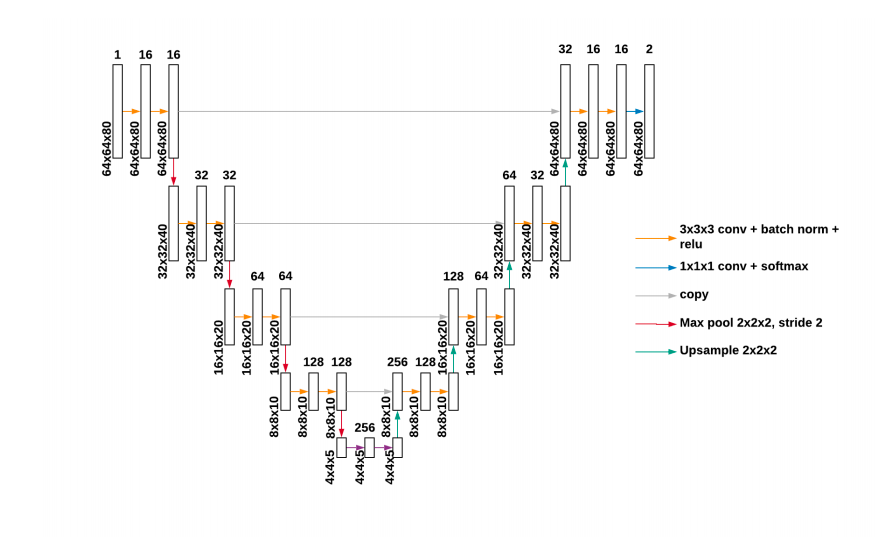
\includegraphics[width=10cm]{images/detection_model.png}
    \caption {Detection Model Architecture}
    \label{fig:detection_model}
\end{figure}
 
\subsection{Detection augmentation}
Unto passing particular batch of scans to detection model each image was represented as 5 cropped samples intruding that at least 4 of them contain some vertebrae pixels. In the meantime each sample scan was sized as $64 \cdot 64 \cdot 80$, meaning 64 pixels by 64 pixels by 80 channels. Withal accordingly each sample has an accompanying dense labelling, containing 0s (for background) and 1s (for vertebrae) of the same size.    
 
\section{Identification Model}
By the previous description, identification model showed on Figure \ref{fig:identification_model} identifies what vertebrates belong which segmented pixels. For what it was established unet-wise architecture with revamped parameters. Updates brought changes of input layer channels number which corresponds to 8 to pass in samples of size $8 \cdot 80 \cdot 320$. The introduced filters sized $5 \cdot 20$ at the lowest level of the architecture  increases the size of the receptive field thereby maximizing the potential information retrieved by the network. To clarify, the background pixels are strained out, denoting just that pixels which are labeled as background when we train model. As for loss function the following modified L1 function was approached:
\begin{align*}
 L = \begin{cases} \lvert y_i - x_i \rvert\ \mbox{if } x\mbox{$\neq 0$} \\ 0, \mbox{ otherwise} \end{cases}
\end{align*}
where $y_i$ - predicted value of pixel $i$ and $x_i$ - true value of pixel $i$.

Unlike standard unet architecture it was used same padding for all convolutional layers with stride 1, a learning rate
$\lambda$ of 0.001, a batch size of 32 and batch normalization after every convolutional layer with momentum of 0.1. The model implementation can be found in project repository. \footnote{\url{https://github.com/KumundzhievMaxim/VertebraeSegmentation/blob/main/train_identification_model.py}}

\begin{figure}[h]
    \centering 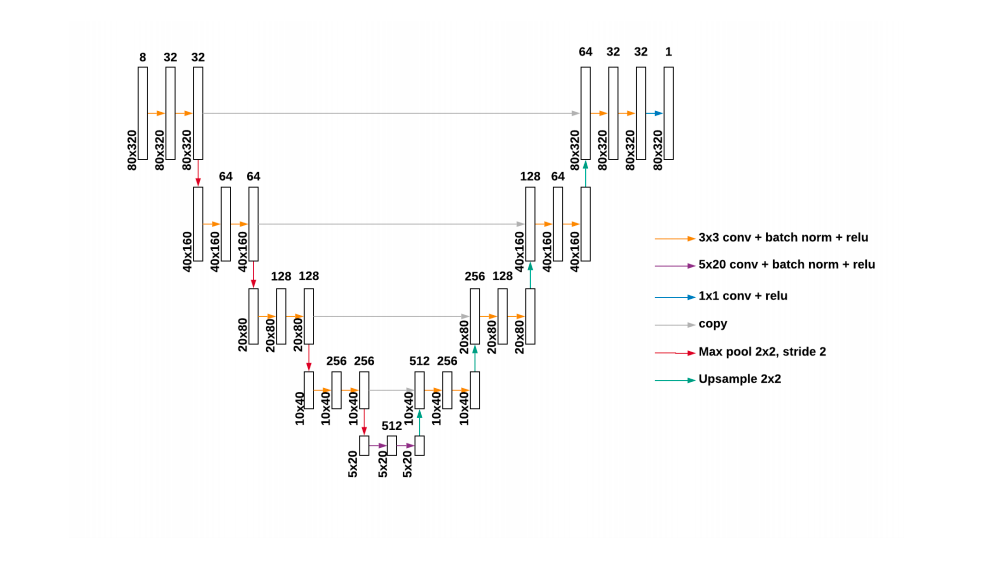
\includegraphics[width=11cm]{images/identification_model.png}
    \caption {Identification Model Architecture}
    \label{fig:identification_model}
\end{figure}

The identification model outputs a continuous value for each pixel of a scan which, is rounded to an integer to correspond to a specific vertebrae. The identification model gives a value to each pixel even if that pixel is not depicting any vertebrae and is a background. These pixels will be filtered out of the final predictions by multiplying them by their corresponding pixel from the output of the detection model which should be 0 for a background pixel. The model outputs are represented as continuous value for each dedicated pixel of particular scan which further is rounded to correspond to a specific vertebrae integer. As well it should be considered the model award each pixel's value nay it is background and does not represent any vertebrae. Even though these pixels will be filtered out of the final predictions by multiplying them by their corresponding pixel from the output of the detection model which should be 0 for a background pixel.

\subsection{Identification augmentation}
Altogether proceeding with identification network for each scan in the training set it was produced 100 cropped samples sized $8 \cdot 80 \cdot 320$ coercing all of them retrieving some vertebrae pixels whereas each with a corresponding dense labelling of size $80 \cdot 320$, representing the labelling for the forth slice of the input sample.

\section{Training models}
To recap input to detection model was initially $64 \cdot 64 \cdot 80$ particular scan which was transformed (5 crops) what afterwards got shape of $32 \cdot 32 \cdot 40$. It worth to mention, jointly training process it was applied padding which discarded the outer border of scan producing $16 \cdot 16 \cdot 20$ shape so far. In simplified terms, it reduced edge artifacts in the detection and led to improved mean localization scores. During roughly 17 hours the detection model had been training for 50 epochs. The validation Dice score achieved 0.911 whereas validation accuracy was 0.985\%. 

In regard of identification model, which was fully CNN the particular input was sized of $8 \cdot 80 \cdot 320$. During roughly 10 hours the identification model had been training for 35 epochs. At test time it was passed whole slices of single input scan, padded to the nearest and multiple of 16.

\section{Inference}
As soon as the identification model outcomes predicted label per each pixel foremost thresholding $x_\upsilon$ is applied as validation whether include particular centroid in the prediction or not by comparing the obtained  number of pixels for a vertebra and assumed thresholding number.

The threshold $x_\upsilon$ is specific to the vertebra $\upsilon$ and formed as:
\begin{align*}
  x_\upsilon = \max(3000, 0.4 \cdot R_\upsilon^3) 
\end{align*}
where R - the radius of the vertebra $v$.

\section{Results}
Moving from left side to right side on the Figure \ref{fig:step_step_predictions} it is represented the single scan evaluation path in terms of each step of full proposed solution pipeline. 

\begin{figure}[h]
    \centering 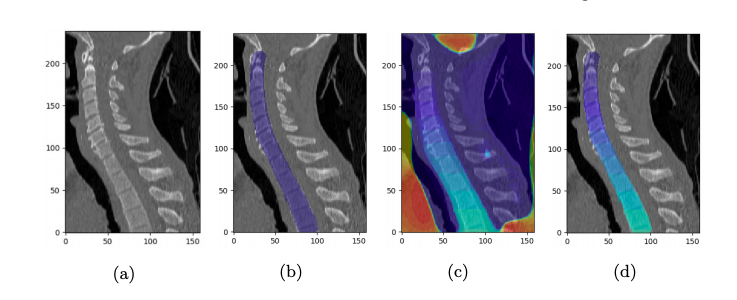
\includegraphics[width=11cm]{images/step_step_predictions.png}
    \caption {(a) shows an original scan in grey scale, (b) shows the output of the detection model applied to the scan, (c) shows the output of the identification model
    applied to the scan, (d) shows (b) and (c) multiplied together to produce a final prediction for each pixel.}
    \label{fig:step_step_predictions}
\end{figure}

As it was mentioned before the resulting measurements have been calculated within testing set of 60 scans of various patient by measured Dice score and metrics as id rate, localization error which derived into mean localization distance error and standard deviation localization distance error.

The 3 resulting random pipeline predictions can be observed at \ref{fig:predictions} figure which represents predictions themselves as well as additional impacting information as ground-truth and localization error. 
\begin{figure}[h]
    \centering 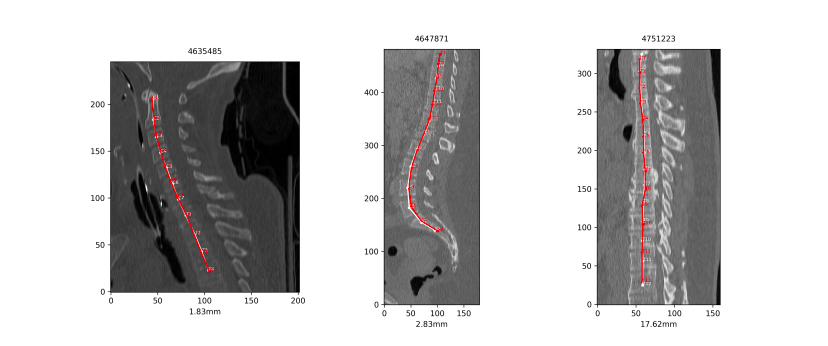
\includegraphics[width=9cm]{images/predictions.png}
    \caption {visualization of 3 random predictions, whereas the red points denote pipeline centroid predictions, the white points denote ground-truth centroid locations. On top of that each scan designated the mean localization error for particular scan.}
    \label{fig:predictions}
\end{figure}

\newpage
\section{Competitors}
As the baseline comparison it was considered "Joint Vertebrae Identification and Localization in Spinal CT Images by Combining Short-Range and Long-Range Contextual Information" work done by Liao at 2018 \cite{Liao2018}. The utilized benchmark architecture is shown on Figure \ref{fig:competitor}.

\begin{figure}[h]
    \centering 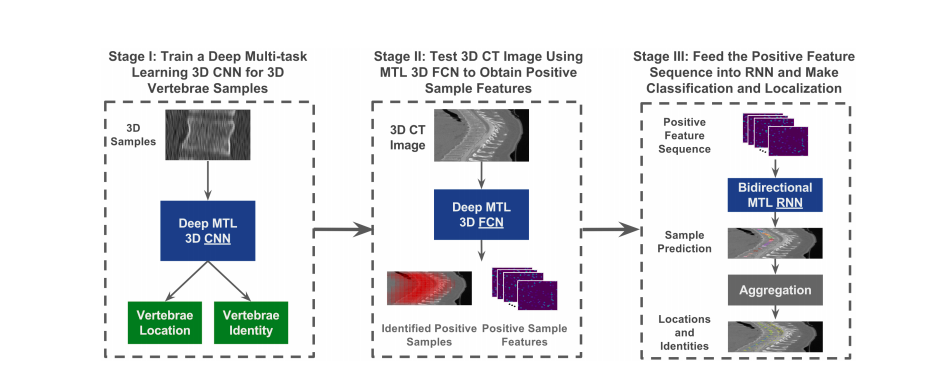
\includegraphics[width=12cm]{images/competitor.png}
    \caption {Overall architecture of the competitor proposed method for vertebrae identification and localization}
    \label{fig:competitor}
\end{figure}

The overall architecture of the proposed method may be traversed as three-stage approach. In the first stage, it was applied deep multi-task 3D CNN using randomly cropped 3D vertebrae samples. Afterwards within second stage transform trained multi-task 3D CNN into a multi-task 3D fully convolutional network by converting the fully connected layers to 3D convolutional layers. Decisively within third stage the extracted sample features will be ordered and form a set of feature sequences. Assimilating the results the following table takes place:


\begin{table}[htbp]
\centering
\begin{tabular}{|l||c|c|} \hline\hline
Metrics & Competitor & 2-stage U-net \\ \hline
Id Rate & 88.3 & 85.8 \\
Mean & 6.47 & 5.60 \\
Std & 8.56 & 7.10 \\
\hline\hline
\end{tabular}
\end{table}

To conclude the models comparison it should mentioned the proposed in this work method does not utilize RNN unlike \cite{Liao2018} work, thus making the method likely more efficient at test time which takes approximately 40 seconds to produce the prediction per single patient scan. 